\documentclass{report}
\usepackage[utf8]{inputenc}
\usepackage[czech]{babel}
\usepackage{graphicx}




\title{Deskriptor}
\author{Kateřina Kratochvílová}

% matematicke rovnice %
\usepackage{amsmath}
%odkazy%
\usepackage{hyperref}

% #########
% # START #
% #########

\begin{document} 
% titulní stránka
%\maketitle
\begin{titlepage}
\begin{flushleft} 
{
\includegraphics[width=.5\textwidth]{./img/fav_logo.jpg}\\[3cm]}
\end{flushleft}
\begin{center}

{\Huge KIV/UIR - Semestrální práce}
\\[0.3cm]
\vspace{1.7cm}
{\Large Kateřina Kratochvílová} \\
\vspace{0.2cm}
{\normalsize dtwok8@students.zcu.cz}\\

{\large \today}
\end{center}
\end{titlepage}


% obsah
\tableofcontents

% abstrakt
\begin{abstract}
abstrakt  
\end{abstract}


\chapter{Poem}
POEM (Patterns of Oriented Edge Magnitudes). Vstup algorimutmu se předpokládá šedotónový obrázek o rozměrech  m x n.

\subsubsection{1. Výpočet gradientu a magnitudy}
Nejprve je potřeba vypočítát gradient. Gradient je obecně směr růstu. Výpočet může probíhat různými způsoby. Pří výpočtu použijeme masku, kterou aplikujeme na vstupní obrázek. Podle některých studii jsou nejlepší jednoduché masky jako je např. $[1, 0, -1]$ a $[1, 0, -1]^{\,t}$. Okraje se buď vypouštějí nebo se dají doplnit (existuje více způsobů doplňění). Výstupem jsou dva obrázky o rozměrech m x n, na výstup se dá pohlíže také jako na vektor, kdy každý bod původního obrázku je reprezentován právě 2D vektorem. Analogicky pokud si vektory rozložíme na x a y složku dostali bychom dva obrázky jeden, který reprezentuje obrázek po použití x-ového filtru, a druhý který reprezentuje obrázek po použití y-filtru. Přičemž použití y filtru by nám mělo zvíraznit hrany v y směru (svislé) a x zvírazní hrany v x směru (vodorovné). Intenzita v každém pixelu představuje velikost gradientu (magnitudu).\\
Magnituda je velikost směru růstu lze si ji představit jako velikost směru růstu pro každý pixel (počítá se tedy pro každý pixel). Počítá se tedy pro každý pixel. Takže se dá počítat jako velikost těch 2D vektrů které jsme dostaly při výpočtu gradientu. Magnituda představuje velikost vektoru gradientu. Magnitudu spočteme jako velikost vektoru.

\begin{align}
	\label{vstupni_matice}image = \begin{pmatrix}8 & 7 & 5 \\1 & 2 & 4 \\3 & 5 & 7 \end{pmatrix}
\end{align}
\begin{align}
	\label{masky}
		maska(x) = \begin{pmatrix}-1 & 1 \end{pmatrix} 
		maska(y) = \begin{pmatrix}-1 \\ 1 \end{pmatrix}
\end{align}

\begin{align}
	\label{vystupni_gradienty}
		gradient(x) = \begin{pmatrix}-1 & -2 & 0\\1 & 2 & 0 \\2 & 2 & 0 \end{pmatrix}
		gradient(y) = \begin{pmatrix}-7 & -5 & -1 \\2 & 3 & 3 \\0 & 0 & 0 \end{pmatrix}
\end{align}

\begin{align}
   \label{velikost_vektoru} |u| = \sqrt{u_1^2 + u_2^2}
\end{align}

\begin{figure}[htp]
	\centering
	\begin{minipage}[c]{150pt}
		\centering
		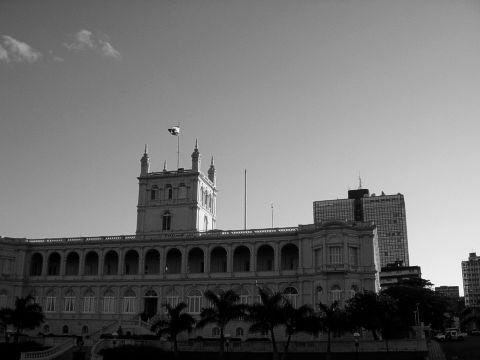
\includegraphics[width=150pt]{./img/vstupni_obraz.jpg}
		\caption{Vstupní obrázek}
	\end{minipage}
	\begin{minipage}[c]{150pt}
		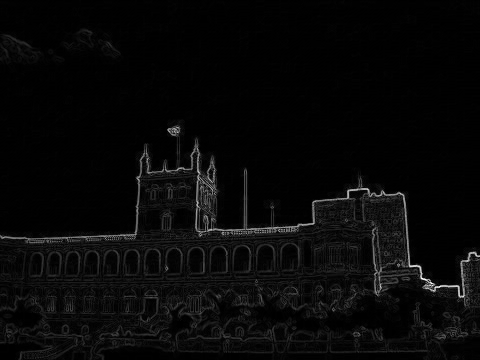
\includegraphics[width=150pt]{./img/magnitude.png}
		\caption{magnituda}
		\centering
	\end{minipage}
\end{figure}

\begin{figure}[htp]
	\centering
	\begin{minipage}[c]{150pt}
		\centering
		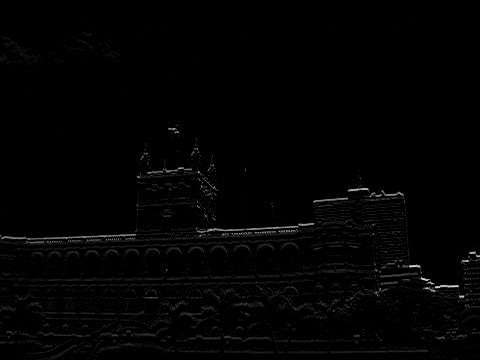
\includegraphics[width=150pt]{./img/gradientX.png}
		\caption{gradient x}
	\end{minipage}
	\begin{minipage}[c]{150pt}
		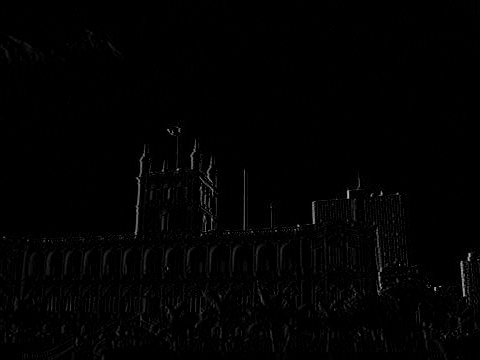
\includegraphics[width=150pt]{./img/gradientY.png}
		\caption{gradient y}
		\centering
	\end{minipage}
\end{figure}

\subsubsection{Diskretizace směru gradientu}
Pokud se na gradienty budeme koukat jako na 2D vektory můžeme určit nejeden jejich velikost(gradient) ale i jejich směr. Je možné použít znamínkovou reprezentaci $0 - \pi$ nebo neznamínkovou reprezentaci $0 - 2\pi$. Každý pixel se pak dá reprezentovat nejen velikostí vektoru ale i jeho směrem. V praxi si rovnoměrně rozdělíme kružnici na několik dílů (podle toho kolik chceme směrů) označme si počet dílů $d$. Pro $d = 3$ znaménkovou reprezentaci to tedy bude $0 - \frac{2}{3}\pi$, $\frac{2}{3}\pi - \frac{4}{3}\pi$ a $\frac{3}{3}\pi - 2\pi$ 

\subsubsection{dalsi}
U každého směru vezmeme každý pixel a jeho okolí a zprůměrujeme jeho hodnoty. Toto okolí se nazývá cell. 

\subsubsection{výpočet LBP}


\begin{figure}[ht]
		\centering
		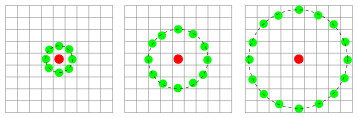
\includegraphics[width=253px]{./img/poem.png}	
		\caption{Znázornění LBP}
\end{figure} \begin{align}
   \label{velikost_vektoru_v_prostoru} |u| = \sqrt{u_1^2 + u_2^2 + u_3^2}
\end{align} 
 
\chapter{Barevný poem}
\begin{align}
   \label{velikost_vektoru_v_prostoru} |u| = \sqrt{u_1^2 + u_2^2 + u_3^2}
\end{align} 

\begin{align}
   \label{soucet_vektrou} \vec{u} + \vec{v} = (u_1 + v_1, u_2 + v_2, u_3 + v_3 )
\end{align} 
 
\section{Textura}
LBP i Gabor pracují s informací o intenzitě obrazu. Detekce hran. Obyčejné LBP problém s rotací.

kombinace textur a barevne informace
1. Vytvoření společného příznaku, 
například rozšíření LBP na všechny barvené kanály
informace o barvě a textuře se mohou oblivňovat protichůdně

2. Vyhodnotit a klasifikovat příznaky odděleně a pak výslednou klasifikaci nějak s pojit z několika částí 
	to je například JEC
	
	výhoda zachovává vlastnosti obou původních příznaků 
	výpočetně náročnější a jeho úspěšnost je přímo závislá na způsobu kombinace obou informací	
	
vutbrno 117319 10 stranka

Gabor filter je lineární filter používaný pro detekci hran. Frekvence a orientace reprezentující Gabor filter je podobná lidskému vnímání a jsou zvláště vhodné pro reprezentaci textury a rozlišování. 

Gabor filtr reaguje na hrany a texturové změny. 

Obrázky jsou filtrovány za použité reálné části z různých odlišních Gabor filtrů jader. Průměrný a rozptyl filtrovaných snímků jsou pak použity jako funkce pro klasifikaci, která je založena na nejméně kvadratické chyby pro jednoduchost.

TODO Dohledat Haar a Gabor wavelety, přidat vzorečky a zase klidně i obrázky

\subsection{Barva}
U digitálního obrazu je barva reprezentovaná n-rozměrným vektorem. Jeho velikost a význam jednotlivých složek (tzv. barevných kanálů) zavisí na příslušném barevném prostoru. Počet bitů použitých k uložení buď celého vektoru nebo jeho jednotlivých složek se nazývá barevná hloubka (totožně bitová hloubka). Obvykle se můžeme setkat s hodnotami 8, 12, 14 a 16 bitů na kanál.
\\
V použité metodě V použité metodě získáme vlastnosti z obrázků ve třech rozdílných barevných prostorech: RGB, HSV a LAB. RGB (Red, Green, Blue) je nejobvykleji používaný pro zachycení obrázu nebo jeho zobrazení. Oproti tomu HSV (Hue, Saturation and Value) se snaží zachytit barevný model tak jak ho vnímá lidské oko, ale zároveň se snaží zůstat jednoduchý na výpočet. Hue znamená odstín barvy, saturation systost barvy a value je hodnota jasu nebo také množství bílého světla. RGB je závislý na konkrétním zařízení, nemůže dosáhnout celého rozsahu barev, které vidí lidské oko, zatímco barevný model LAB je shopen obsáhnout celé viditelné spektrum a navíc je nezávislý na zařízení. L (ve zkratce LAB) značí Luminanci (jas dosahuje hodnot 0 - 100, kde 0 je černá a 100 je bílá). Zbylé A a B jsou dvě barvonosné složky, kdy A je ve směru červeno/zeleném a B se pohybuje ve směru modro/žlutém. 
\\
Pro RGB, HSV i LAB použijeme barevnou hloubku 16 bitů na kanál histogramu v jejich příslušném barevném prostoru. 

Jako reprezentace textur budou použity Gabor a Haar wavelety. Každý obrázek bude filtrován s Gabor wavelet na třech škálách a čtyřech orientacích. 


\chapter{Použité programové prostředky}
Program byl navržen na operační systému Linux. Jako programovací jazyk byl zvolen Python a to z důvodu jeho jednoduchého použití, což je na prototyp, jako je tento velice výhodné na časovou náročnost. Program využívá knihovnu OpenCV 3.1. 
  
\section{OpenCV}
OpenCV (Open source computer vision) je knihovna vydávána pod licencí BSD a je volně k dispozici jak pro akademické účely, tak pro komerční použití. Je vhodná pro použití v C++, C, Python a Javě. Podporuje operační systémy Windows, Linux, Mac OS, iOS a Android.
\\
Knihovna byla navrhnuta pro výpočetní efektivitu v oblasti počítačového vidění a zpracování obrazu se zaměřením na zpracování obrazu v reálném čase. Z důvodu optimalizace byla napsána v C/C++. 
\\
Knihovnu OpenCV je možné stáhnout na adrese: http://opencv.org/

\chapter{Závěr}
V teoretické části byly popsány nízkoúrovňové příznaky barva a textura. Byla rozebrána metoda JEC, která bude v bakalářské práci implementována. Seznamili jsme se s knihovnou OpenCV, prostudovali obrázk y apříložená metadata.

\chapter{Uživatelská dokumentace}
popsani jak vypada zdrojovej soubor kterej to zere, nejdriv cesta k souboru a pak jeho klicovy slova

\chapter{Zdroje}
\url{https://dspace5.zcu.cz/bitstream/11025/17883/1/A13N0110P.pdf} \\
\url{https://en.wikipedia.org/wiki/Local_binary_patterns} \\

\end{document}